Bộ nhớ tái phát có thể được xem xét là một phiên bản đơn giản của bộ nhớ dài-ngắn hạn. Đối với bộ nhớ dài-ngắn hạn, nó điều chỉnh trực tiếp lượng thông tin của trạng thái ẩn bằng cổng quên và cổng đầu ra, còn bộ nhớ tái phát chỉ sử dụng một cổng đặt lại (\textit{reset gate}). Điểm khác biệt lớn là bộ nhớ tái phát không dùng ô trạng thái làm bộ nhớ.
\begin{figure}[htb]
    \centering
    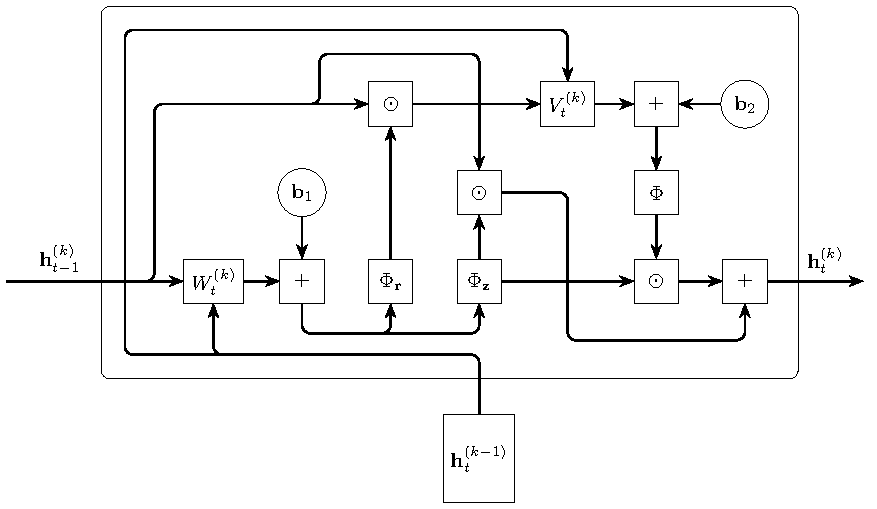
\includegraphics[width=0.7\textwidth]{tikz_image/gru_architecture.pdf}
    \caption{Kiến trúc của GRU}
    \label{fig:gru-architecture}
\end{figure}

Xét một nút ẩn bất kỳ trong mạng thần kinh nhiều lớp, thay vì phải tính đến bốn vector trung gian thì bộ nhớ tái phát chỉ tính hai vector trung gian là cổng đặt lại và cổng cập nhật (\textit{update gate})
\begin{align}
    \begin{bmatrix}
        \mathbf z \\
        \mathbf r
    \end{bmatrix}
     & =
    \begin{pmatrix}
        \text{sigmoid} \\
        \text{sigmoid}
    \end{pmatrix}
    \left(W^{(k)}_t
    \begin{bmatrix}
            \mathbf h_{t}^{(k-1)} \\
            \mathbf h_{t-1}^{(k)}
        \end{bmatrix}
    +\mathbf b_1\right)
     & [\text{Tính các vector trung gian}]                                 \\
    \mathbf h_t^{(k)}
     & =\mathbf z\odot\mathbf h_{t-1}^{(k)}+(\mathbf 1-\mathbf z)\odot\Phi
    \left(V^{(k)}_t
    \begin{bmatrix}
            \mathbf h_{t}^{(k-1)} \\
            \mathbf r\odot\mathbf h_{t-1}^{(k)}
        \end{bmatrix}
    +\mathbf b_2\right)
     & [\text{Tính trạng thái ẩn}]
\end{align}

Ma trận $W_t^{(k)}$ bây giờ chỉ có số chiều là $2p\times 2p$ vì nó chỉ cần tạo ra hai vector trung gian ở đầu ra, còn ma trận $V_t^{(k)}$ sẽ có số chiều là $p\times 2p$. Vì bộ nhớ tái phát không sử dụng ô trạng thái để làm bộ nhớ, nên hai cổng của nó phải đảm nhiệm nhiệm vụ này. Bộ nhớ tái phát hoạt động qua hai bước như sau:
\begin{enumerate}
    \item Tính các vector trung gian $\mathbf{z,r}$
    \item Tại bước tính trạng thái ẩn $\mathbf h_t^{(k)}$ sẽ có hai việc xảy ra
          \begin{itemize}
              \item Cổng đặt lại $\mathbf r$ sẽ quyết định có bao nhiêu dữ liệu cũ được truyền vô trạng thái ẩn $\mathbf r\odot\mathbf h_{t-1}^{(k)}$, và nó sẽ thông qua một phép nhân ma trận $V$ để kết hợp trạng thái ẩn từ lớp thời gian trước đó $\mathbf h_{t-1}^{(k)}$ với trạng thái ẩn từ lớp trước đó $\mathbf h_{t}^{(k-1)}$ với nhau.
              \item Cổng cập nhật $\mathbf z$ xem tổng đóng góp của hai trạng thái ẩn (trạng thái ẩn từ lớp thời gian trước đó $\mathbf h_{t-1}^{(k)}$ và kết quả vừa tính ở bước trên) là bằng $1$. Cổng cập nhật sẽ chia ra hai phần $\mathbf z$ và $1-\mathbf z$ như là phần bù của nhau để quyết định sẽ lấy dữ liệu của mỗi bên đóng góp như thế nào.
          \end{itemize}
\end{enumerate}

Như có thể thấy cổng cập nhật làm hai nhiệm vụ, đầu tiên là hoạt động giống như một cổng đầu vào $\mathbf z$, thứ hai là hoạt động giống như một cổng quên $1-\mathbf z$. Xét một bộ nhớ tái phát với duy nhất một lớp với $v_1,v_2$ là hai trọng số của ma trận $V$, ta có
\begin{align}
    h_t=z\cdot h_{t-1}+(1-z)\cdot\Phi(v_1x_t+v_2rh_{t-1}+b)
\end{align}
Đạo hàm giữa hai nút trong bộ nhớ tái phát sẽ là
\begin{align}
    \dfrac{\partial h_t}{\partial h_{t-1}}=z+v_2r(1-z)\cdot\Phi'
\end{align}
Như đã nói dòng chảy của đạo hàm trong lan truyền ngược sẽ phụ thuộc vào đạo hàm giữa hai nút kề nhau. Thành phần $z\in(0,1)$ sẽ làm cho lan truyền này ổn định hơn vì nó làm cho đạo hàm khó bằng $0$. Ngoài ra khi $z$ quá nhỏ thì thành phần $(1-z)$ sẽ đóng vai trò của $z$ trong trường hợp trên, và nó là thành phần làm cho dòng chảy này ổn định, nên tổng của hai thành phần này sẽ làm cho đạo hàm xấp xỉ $1$. Điều đó giải quyết vấn đề độ dốc biến mất trong mạng thần kinh.
